\documentclass[a4paper, oneside, final]{memoir}
\usepackage[T1]{fontenc}
\usepackage[utf8]{inputenc}
\usepackage[british]{babel}
\usepackage{amsmath}
\usepackage{amsthm}
\usepackage{ifthen}
\usepackage{verbatim}
\usepackage{multirow}
\renewcommand{\rmdefault}{ugm}

% bedre orddeling Gør at der som minimum skal blive to tegn på linien ved
% orddeling og minimum flyttes to tegn ned på næste linie. Desværre er værdien
% anvendt af babel »12«, hvilket kan give orddelingen »h-vor«.
\renewcommand{\britishhyphenmins}{22} 

% Fix of fancyref to work with memoir. Makes references look
% nice. Redefines memoir \fref and \Fref to \refer and \Refer.
% \usepackage{refer}             %
% As we dont really have any use for \fref and \Fref we just undefine what
% memoir defined them as, so fancyref can define what it wants.
\let\fref\undefined
\let\Fref\undefined
\usepackage{fancyref} % Better reference. 

\usepackage{pdflscape} % Gør landscape-environmentet tilgængeligt
\usepackage{fixme}     % Indsæt "fixme" noter i drafts.
\usepackage{hyperref}  % Indsæter links (interne og eksterne) i PDF

\usepackage[format=hang]{caption,subfig}
\usepackage{graphicx}
\usepackage{stmaryrd}
\usepackage{amssymb}
\usepackage{listings}
\usepackage{ulem} % \sout - strike-through
\usepackage{tikz}

%\renewcommand{\ttdefault}{txtt} % Bedre typewriter font
% \usepackage[sc]{mathpazo}     % Palatino font
%\renewcommand{\rmdefault}{urw-garamond} % Garamond
%\usepackage[urw-garamond]{mathdesign}

% \overfullrule=5pt
% \setsecnumdepth{part}
\setcounter{secnumdepth}{1} % Sæt overskriftsnummereringsdybde. Disable = -1.
\setlength{\parskip}{0.25in}

\title{Statistical Methods for Machine Learning\\Case 2}

\author{Troels Henriksen (athas@sigkill.dk) \\ Daniel Fairchild
  (daniel.fairchild@gmail.com)}

\date{\today}
\pagestyle{plain}

\newcommand{\nfrac}[2]{\frac{\displaystyle{#1}}{\displaystyle{#2}}}

\begin{document}

\maketitle

We have never used R before, so for the novelty, that is the language
we have decided to use for this assignment.

\section*{Question 1.1}

The code for this question is in \texttt{src/1112.R}.  The
pseudoinverse function had to be written from scratch, as we could not
find the library supposed to contain it.  We obtained the following
results.

\begin{tabular}{|l|r|}
  \textbf{Selection} & \textbf{RMS error} \\\hline
  1 & 4.944719 \\\hline
  2 & 6.880314
\end{tabular}

Selection 1 appears to have the smaller error compared to the true
results, which is expected as its model incorporates more measurements
than selection 2.  While body measurements are probably only slightly
independent, adding more still constitutes a net information increase.
\newpage
\section*{Question 1.2}

The code for this question is in \texttt{src/1112.R}.

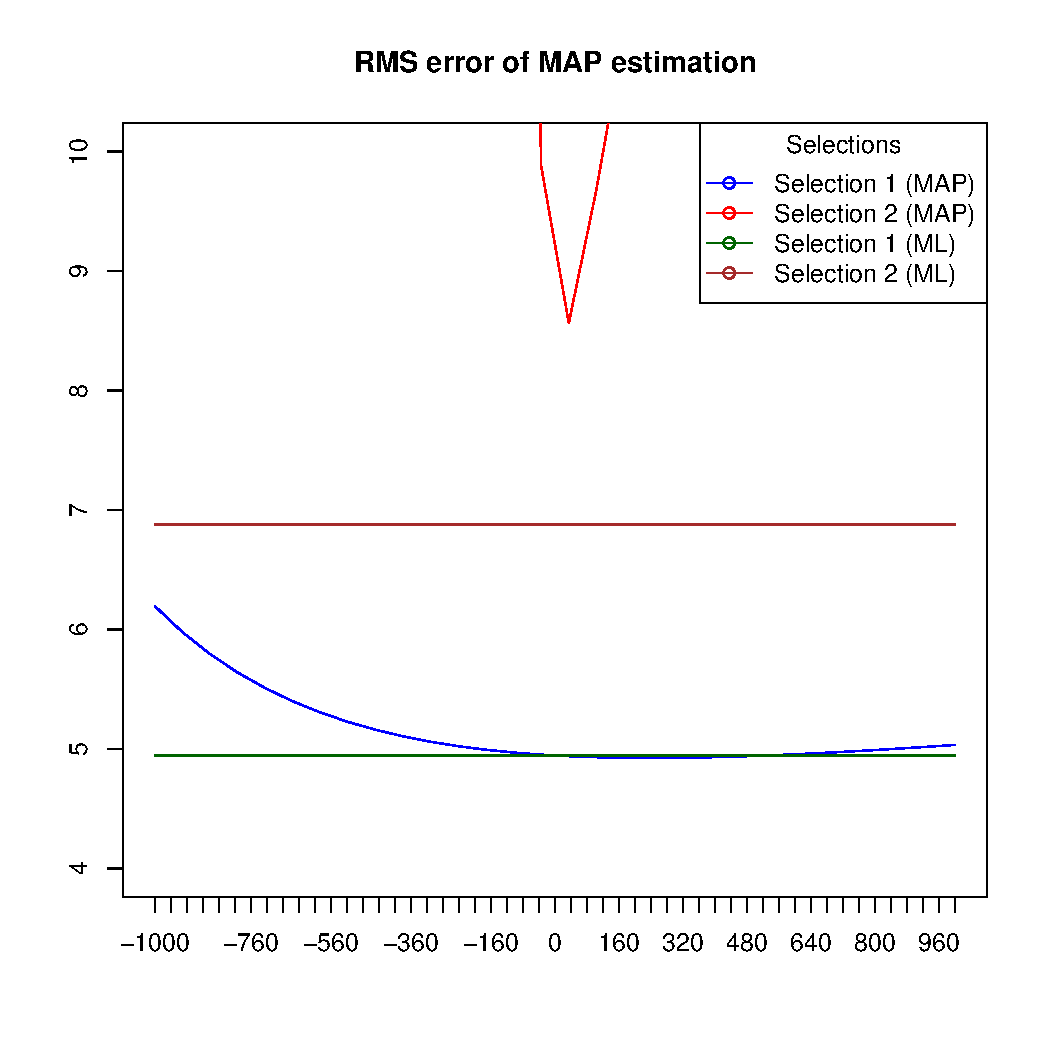
\includegraphics[width=10cm]{img/question12-plot.pdf}

Below is a close-up of the ML estimate and the MAP estimate.

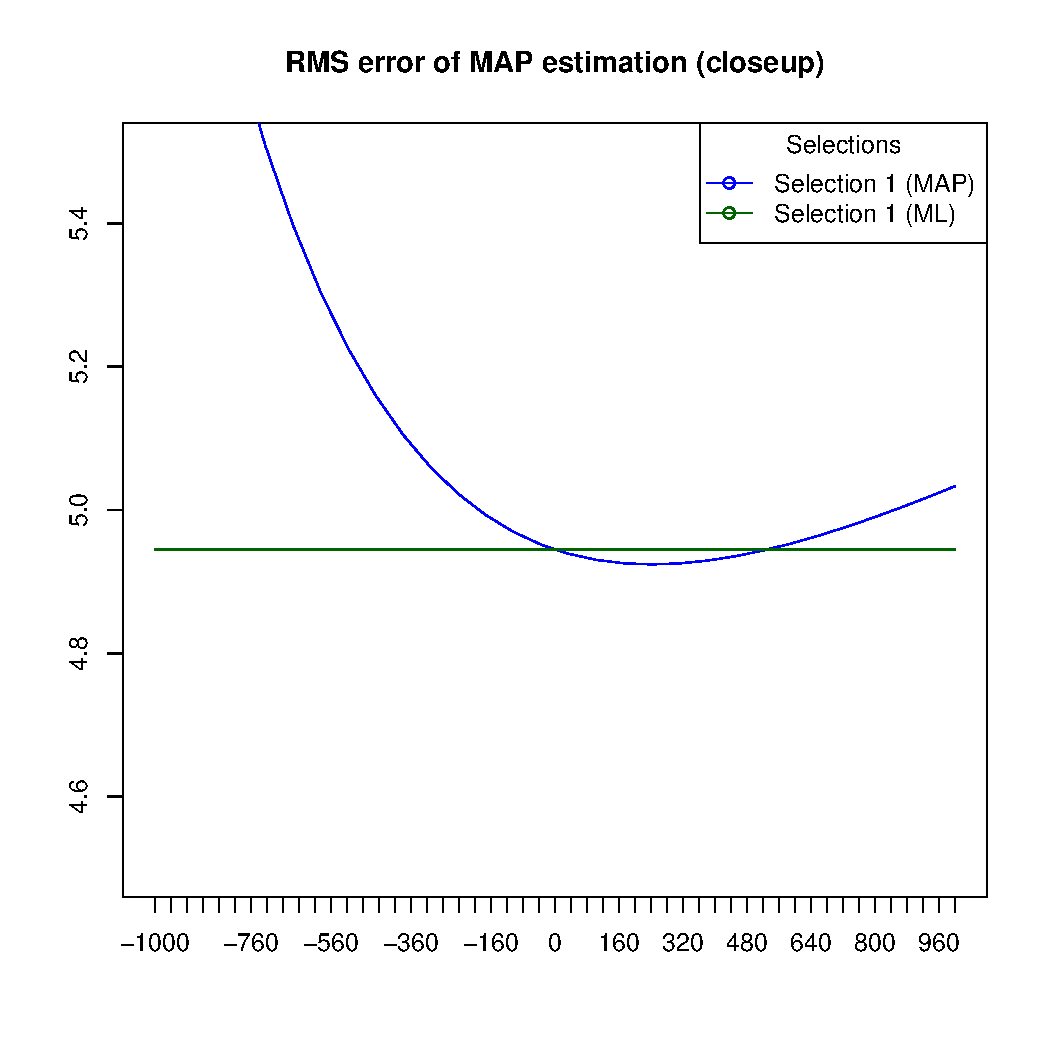
\includegraphics[width=10cm]{img/question12-plot-b.pdf}

We see that the MAP estimate has a slightly smaller error when the
prior precision is in the interval from roughly 0 to 500.

\section*{Question 2}

The code for this question is in \texttt{src/2.R}.

\subsection*{Visualisation}
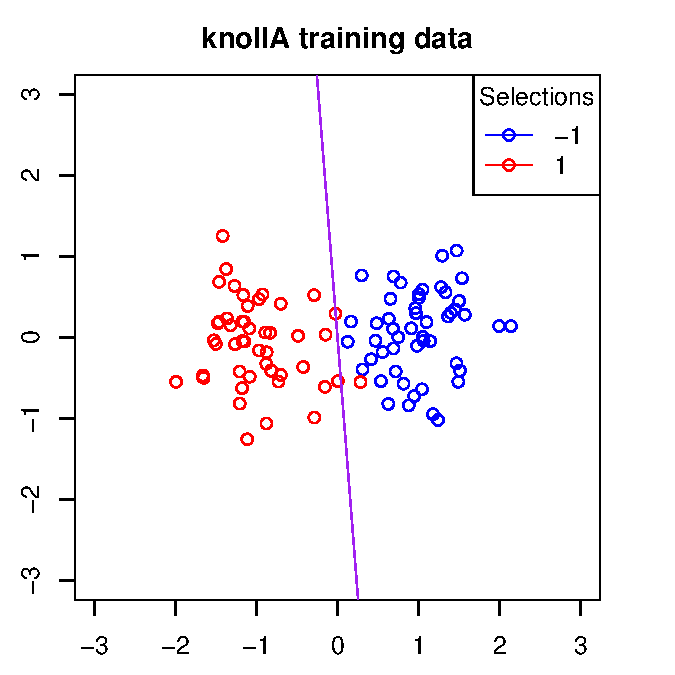
\includegraphics[width=5cm]{img/question2-plot-a.pdf}
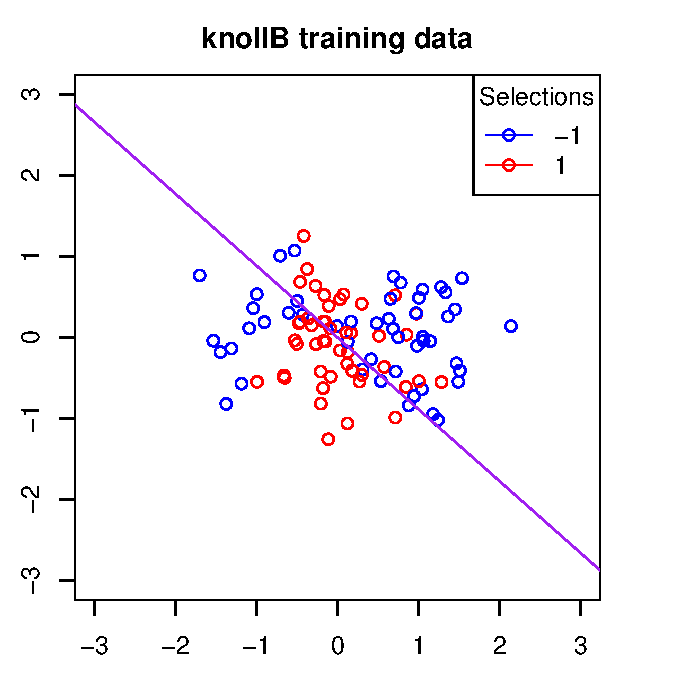
\includegraphics[width=5cm]{img/question2-plot-b.pdf}
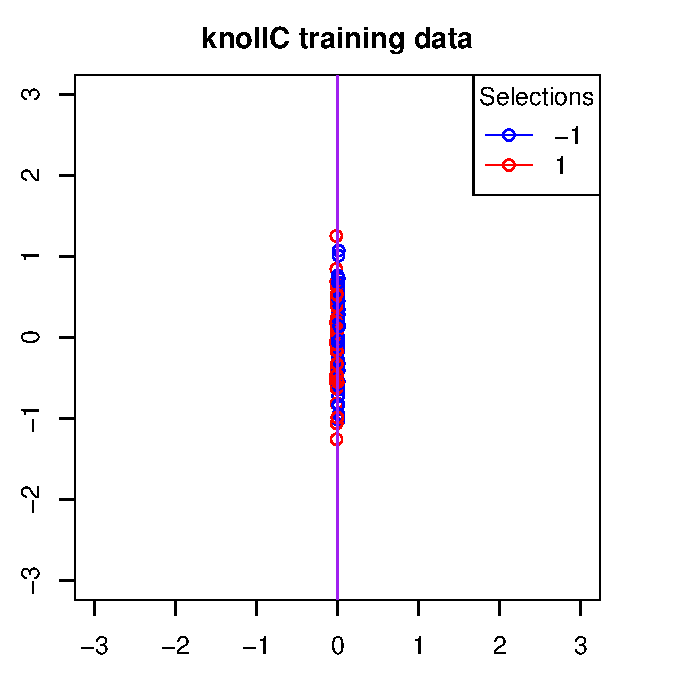
\includegraphics[width=5cm]{img/question2-plot-c.pdf}

\subsection*{LDA}

Let class $\mathcal{C}_1$ be the class indexed by $1$ and
$\mathcal{C}_2$ the class indexed by $-1$.  We have chosen to make use
of Fisher's linear discriminant, as sescribed in section 4.1.4 in the
textbook, implemented in R.  $y$ is classified as class
$\mathcal{C}_1$ if $y\geq 0$ and otherwise class $\mathcal{C}_2$ -
this threshold is based on the idea that we pick the class that our
prediction is closest to.  The class dividers are visualised as purple
lines in the plots.  The accuracy of the linear model is determined by
counting the number of correct classifications proportional to the
number of data points.

\begin{tabular}{|l|l|l|}
  \textbf{Trained with} & \textbf{Tested on} & \textbf{Accuracy} \\\hline
  \multirow{2}{*}{KnollA} & Training set & 0.99 \\
  & Testing set & 0.97 \\\hline
  \multirow{2}{*}{KnollB} & Training set & 0.63 \\
  & Testing set & 0.49 \\\hline
  \multirow{2}{*}{KnollC} & Training set & 0.99 \\
  & Testing set & 0.97 \\\hline
\end{tabular}

We note that the first coordinates in the KnollA and KnollC data sets
are proportional by a factor of 100, hence their identical behaviour.
This is visualised in the plot below.  Due to this similarity we will
focus only on KnollA and KnollB.

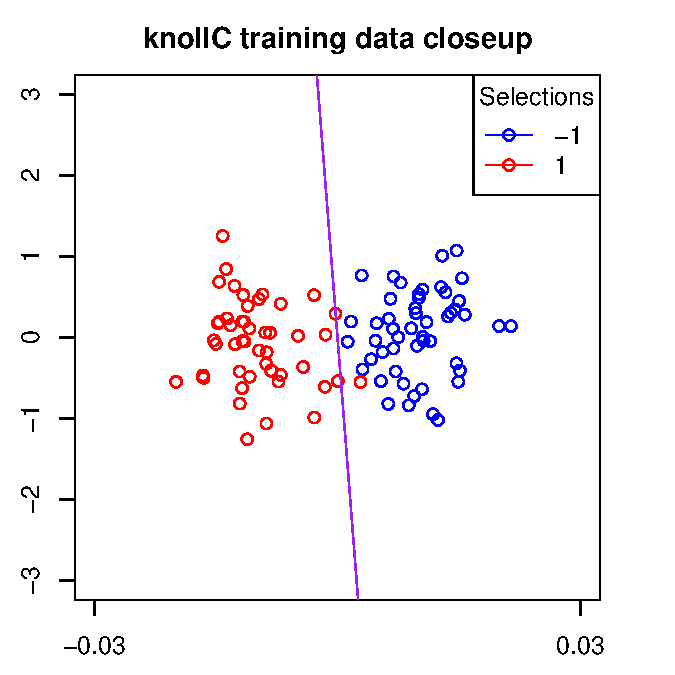
\includegraphics[width=5cm]{img/question2-plot-c-close.pdf}

The difference in accuracy between the KnollA and KnollB data sets can
be visualised by inspecting the distribution of points in KnollB.  It
is immediately clear that there is no way to divide the
two-dimensional plane with a straight line, such that we will obtain a
satisfactory division of the points into their correct classes.  On
the other hand, it is likely that a nonlinear method could construct a
curve that would perform such a division, as the red points do seem to
be clustered roughly in the middle.

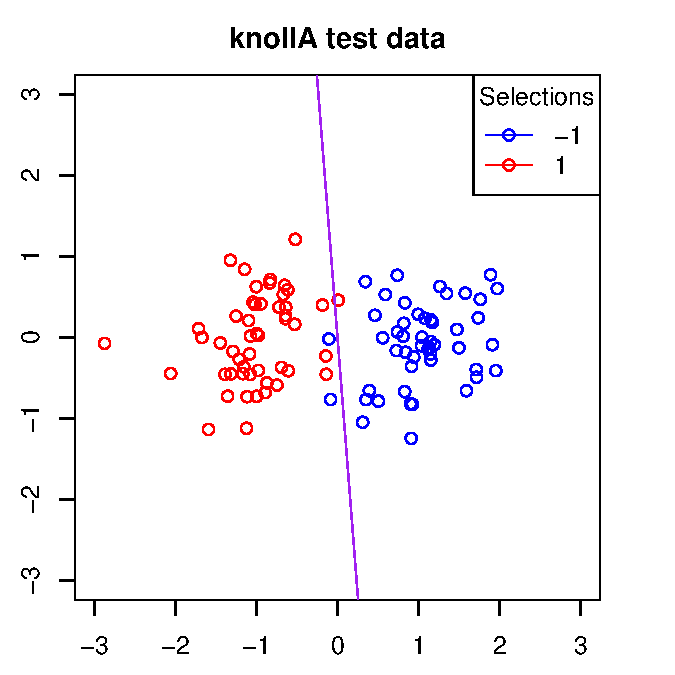
\includegraphics[width=5cm]{img/question2-plot-test-a.pdf}
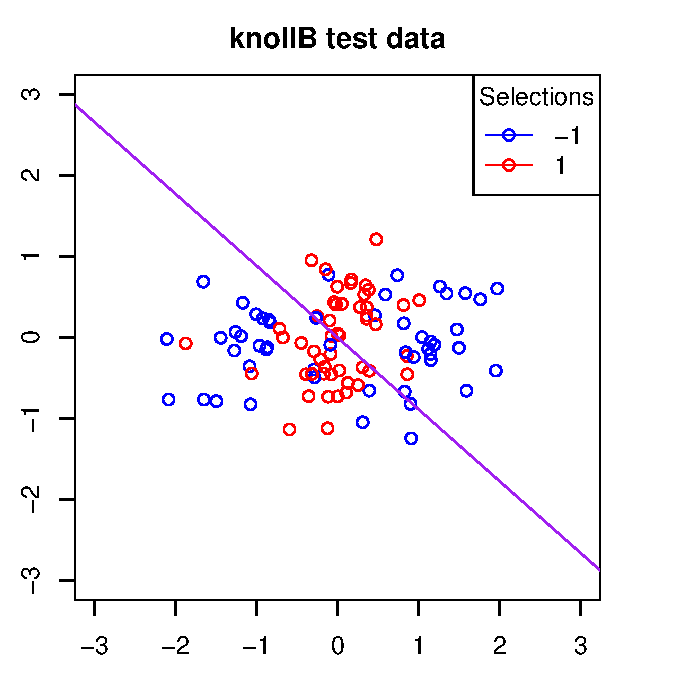
\includegraphics[width=5cm]{img/question2-plot-test-b.pdf}

\newpage
\section*{Question 3.2}

We check that the given metric fulfills the four requirements for a
metric, utilising the properties of norms.

\begin{enumerate}
\item $d(\bold{x},\bold{z}) \geq 0$ (non-negativity): As a norm
  $||\cdot||$ is always non-negative, this property is immediate.
\item $d(\bold{x},\bold{z}) = 0 \Leftrightarrow \bold{x}=\bold{z}$ (identity of
  indiscernibles): The norm $||\bold{Mx}-\bold{Mz}||$ is only zero if
  $\bold{Mx}-\bold{Mz}=\bold{0}$ (by the definition of a norm), which
  is again only the case if $\bold{x}=\bold{z}$.  Holds in both
  directions.
\item $d(\bold{x},\bold{z}) = d(\bold{z},\bold{x})$ (symmetry):
  \begin{align*}
    d(\bold{x},\bold{z})&=||\bold{Mx}-\bold{Mz}||&\text{(By def.)} \\
    &=||\bold{Mx}+(-1)\bold{Mz}||&\text{(Rewriting)} \\
    &=||(-1)\bold{Mz}+\bold{Mx}||&\text{(Commutativity of addition)} \\
    &=|-1|||(-1)\bold{Mz}+\bold{Mx}||&\text{(Multiplying by one)} \\
    &=||\bold{Mz}-\bold{Mx}||&\text{(Positive homogeneity of norms)} \\
    &=d(\bold{z},\bold{x})&\text{(By def.)}
\end{align*}
\item $d(\bold{x}, \bold{z}) \leq d(\bold{x}, \bold{y}) + d(\bold{y},
  \bold{z})$ (triangle inequality):
  \begin{align*}
    ||\bold{Mx}-\bold{My}+\bold{My}-\bold{Mz}|| &\leq ||\bold{Mx}-\bold{My}|| + ||\bold{My}-\bold{Mz}||&\text{(By triangle ineq. of norms)}\\
    ||\bold{Mx}-\bold{Mz}|| &\leq ||\bold{Mx}-\bold{My}|| + ||\bold{My}-\bold{Mz}||&\text{(Simplifying terms)}\\
    d(\bold{x}, \bold{z}) &\leq d(\bold{x}, \bold{y}) + d(\bold{y}, \bold{z})&\text{(By def.)}
  \end{align*}
\end{enumerate}\qed

\end{document}
